% Using a template from https://www.iacr.org/authors/tikz/

\documentclass{standalone}

\usepackage{tikz}
\usepackage{amssymb}

\usetikzlibrary{calc}

%X coordinates for each branch
\newcommand\XA{0.5}
\newcommand\XB{2}
\newcommand\XC{3.5}
\newcommand\XD{5}

%starting Y coordinate for nodes
\newcommand\Y{12}

%vertical distance between nodes
\newcommand\dY{0.7}

\begin{document}
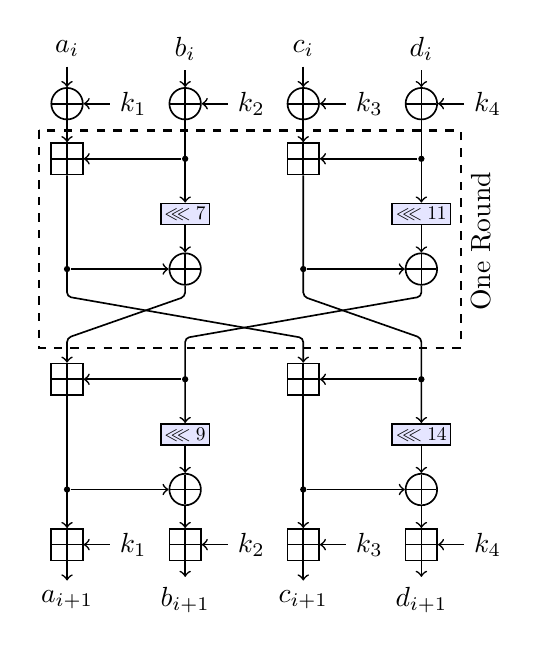
\begin{tikzpicture}
  [line width=0.6,trim left,
   shiftbox/.style = {
     draw, fill=blue!10, 
     inner xsep=0.05cm, inner ysep=0.05cm,
   },
   wire/.style = {
     rounded corners=1.5pt
   },
   xor/.style = {
      draw, circle, inner sep=0cm, minimum size=0.4cm,
      append after command = {
         [shorten >=\pgflinewidth, shorten <=\pgflinewidth,]
        (\tikzlastnode.north) edge (\tikzlastnode.south)
        (\tikzlastnode.east) edge (\tikzlastnode.west)
     }
   },
   oplus/.style = {
      draw, rectangle, inner sep=0cm, minimum size=0.4cm,
      append after command = {
       [shorten >=\pgflinewidth, shorten <=\pgflinewidth,]
       (\tikzlastnode.north) edge (\tikzlastnode.south)
       (\tikzlastnode.east) edge (\tikzlastnode.west)
     }     
   },
   dot/.style = {
     fill, circle, inner sep=0cm, minimum size=0.08cm
   }]

  \node at (\XA, \Y) (a) {$a_i$};
  \node at (\XB, \Y) (b) {$b_i$};
  \node at (\XC, \Y) (c) {$c_i$};
  \node at (\XD, \Y) (d) {$d_i$};

	% Input key whitening.
	\node[xor] at (\XA, \Y-1*\dY) (k1A) {};
	\node[xor] at (\XB, \Y-1*\dY) (k1B) {};
	\node[xor] at (\XC, \Y-1*\dY) (k1C) {};
	\node[xor] at (\XD, \Y-1*\dY) (k1D) {};

	\node at (\XA + 1.2*\dY, \Y-1*\dY) (k1top) {$k_1$};
	\node at (\XB + 1.2*\dY, \Y-1*\dY) (k2top) {$k_2$};
	\node at (\XC + 1.2*\dY, \Y-1*\dY) (k3top) {$k_3$};
	\node at (\XD + 1.2*\dY, \Y-1*\dY) (k4top) {$k_4$};
	\draw[wire, ->] (k1top) -- (k1A);
	\draw[wire, ->] (k2top) -- (k1B);
	\draw[wire, ->] (k3top) -- (k1C);
	\draw[wire, ->] (k4top) -- (k1D);

	% Mix 1
	\node[oplus] at (\XA, \Y-2*\dY) (op1A) {};
	\node[dot] at (\XB, \Y-2*\dY) (op1Adot) {};
	\node[shiftbox] at (\XB, \Y-3*\dY) (op1B) {\scalebox{0.7}{$\lll 7$}}; % 17
	\node[xor] at (\XB, \Y-4*\dY) (op1C) {};
	\node[dot] at (\XA, \Y-4*\dY) (op1Cdot) {};
	% Mix 2
	\node[oplus] at (\XC, \Y-2*\dY) (op2A) {};
	\node[dot] at (\XD, \Y-2*\dY) (op2Adot) {};
	\node[shiftbox] at (\XD, \Y-3*\dY) (op2B) {\scalebox{0.7}{$\lll 11$}}; % 20
	\node[xor] at (\XD, \Y-4*\dY) (op2C) {};
	\node[dot] at (\XC, \Y-4*\dY) (op2Cdot) {};

	\draw[thick,dashed] ($(op1A.north west)+(-0.15,0.15)$) rectangle ($(op2C.south east)+(0.35,-0.85)$);
	\node[rotate=90] at (\XD+0.75, \Y-3.5*\dY) (rectlabel) {One Round};

	% Mix 3
	\node[oplus] at (\XA, \Y-6*\dY) (op3A) {};
	\node[dot] at (\XB, \Y-6*\dY) (op3Adot) {};
	\node[shiftbox] at (\XB, \Y-7*\dY) (op3B) {\scalebox{0.7}{$\lll 9$}}; % 9
	\node[xor] at (\XB, \Y-8*\dY) (op3C) {};
	\node[dot] at (\XA, \Y-8*\dY) (op3Cdot) {};
	% Mix 4
	\node[oplus] at (\XC, \Y-6*\dY) (op4A) {};
	\node[dot] at (\XD, \Y-6*\dY) (op4Adot) {};
	\node[shiftbox] at (\XD, \Y-7*\dY) (op4B) {\scalebox{0.7}{$\lll 14$}}; % 30
	\node[xor] at (\XD, \Y-8*\dY) (op4C) {};
	\node[dot] at (\XC, \Y-8*\dY) (op4Cdot) {};

	% Output key whitening.
	\node[oplus] at (\XA, \Y-9*\dY) (k2A) {};
	\node[oplus] at (\XB, \Y-9*\dY) (k2B) {};
	\node[oplus] at (\XC, \Y-9*\dY) (k2C) {};
	\node[oplus] at (\XD, \Y-9*\dY) (k2D) {};

	\node at (\XA + 1.2*\dY, \Y-9*\dY) (k1bot) {$k_1$};
	\node at (\XB + 1.2*\dY, \Y-9*\dY) (k2bot) {$k_2$};
	\node at (\XC + 1.2*\dY, \Y-9*\dY) (k3bot) {$k_3$};
	\node at (\XD + 1.2*\dY, \Y-9*\dY) (k4bot) {$k_4$};
	\draw[wire, ->] (k1bot) -- (k2A);
	\draw[wire, ->] (k2bot) -- (k2B);
	\draw[wire, ->] (k3bot) -- (k2C);
	\draw[wire, ->] (k4bot) -- (k2D);

  % Final output
  \node at (\XA, \Y-10*\dY) (at) {$a_{i+1}$};
  \node at (\XB, \Y-10*\dY) (bt) {$b_{i+1}$};
  \node at (\XC, \Y-10*\dY) (ct) {$c_{i+1}$};
  \node at (\XD, \Y-10*\dY) (dt) {$d_{i+1}$};

	% Draw all vertical wires.
	\draw[wire, ->] (a) -- (k1A);
	\draw[wire, ->] (b) -- (k1B);
	\draw[wire, ->] (c) -- (k1C);
	\draw[wire, ->] (d) -- (k1D);

	\draw[wire, ->] (k2A) -- (at);
	\draw[wire, ->] (k2B) -- (bt);
	\draw[wire, ->] (k2C) -- (ct);
	\draw[wire, ->] (k2D) -- (dt);


	\draw[wire, ->] (k1A) -- (op1A);
	\draw[wire, ->] (k1B) -- (op1B);
	\draw[wire, ->] (k1C) -- (op2A);
	\draw[wire, ->] (k1D) -- (op2B);

%	\draw[wire, ->] (op1A) -- (op3A);
	\draw[wire, ->] (op1A) -- ($(op1A) + (0, -2.5*\dY)$) -- ($(op4A) + (0, +0.75*\dY)$) -- (op4A);
	\draw[wire, ->] (op1B) -- (op1C); % Internal to mix
%	\draw[wire, ->] (op1C) -- (op3B);
	\draw[wire, ->] (op1C) -- ($(op1C) + (0, -0.5*\dY)$) -- ($(op3A) + (0, +0.75*\dY)$) -- (op3A);
%	\draw[wire, ->] (op2A) -- (op4A);
	\draw[wire, ->] (op2A) -- ($(op2A) + (0, -2.5*\dY)$) -- ($(op4B) + (0, +1.75*\dY)$)-- (op4B);
	\draw[wire, ->] (op2B) -- (op2C); % Internal to mix
%	\draw[wire, ->] (op2C) -- (op4B);
	\draw[wire, ->] (op2C) -- ($(op2C) + (0, -0.5*\dY)$) -- ($(op3B) + (0, +1.75*\dY)$) -- (op3B);

	\draw[wire, ->] (op3A) -- (k2A);
	\draw[wire, ->] (op3B) -- (op3C); % Internal to mix
	\draw[wire, ->] (op3C) -- (k2B);
	\draw[wire, ->] (op4A) -- (k2C);
	\draw[wire, ->] (op4B) -- (op4C); % Internal to mix
	\draw[wire, ->] (op4C) -- (k2D);

	% Draw horizontal lines.
	\draw[wire, ->] (op1Adot) -- (op1A);
	\draw[wire, ->] (op2Adot) -- (op2A);
	\draw[wire, ->] (op3Adot) -- (op3A);
	\draw[wire, ->] (op4Adot) -- (op4A);

	\draw[wire, ->] (op1Cdot) -- (op1C);
	\draw[wire, ->] (op2Cdot) -- (op2C);
	\draw[wire, ->] (op3Cdot) -- (op3C);
	\draw[wire, ->] (op4Cdot) -- (op4C);

\end{tikzpicture}
\end{document}
